\section{Introduction}
There has always been a need to be able to take human readable input, and generate output from it, whether it be for generating graphs, typesetting documents, or creating computer programs. The problem of turning human input into a meaningful data structure readable by programs has always been a difficult issue. Programs called \textit{``compilers''} were designed to solve this problem. Noam Chomsky's 1956 paper \textit{``Three Models For The Description Of Language''} redefined how to solve formal languages, becoming a fundamental paper in the field. \textit{``Compilers Principles Techniques and Tools''} is considered the strongest source available in terms of compiler design, with \textit{``Parsing Techniques - A Practical Guide''} going into greater depth about \textit{``parsing''}, the idea of turning human readable input into meaningful data structures.

\newpage
\section{Language Parsing Design}

\subsection{Determining how to parse the syntax of a language}
A formal language is defined as a set of strings of symbols for use in situations where a natural language(such as English) isn't suitable eg. Mathematics, and Computer programming. Where each symbol has precise semantic, and syntactic relation to each other. Writing formal grammar rules uses a set of finite \textit{``productions''}. Productions, are rules that signify substitution of symbols within a string, there are typically three symbols when writing productions in formal grammars. Productions rules are used show how a compiler will take strings, and convert them into tokens. These tokens are then sorted into a hierarchy that can be used by the next stage of the compiler. The \textit{|}, known as the vertical bar or \textit{``pipe''} symbol, is used to symbolise a grouping of rules applying to the same rule.
\begin{description}
    \item[\textit{Terminal Symbols}] Symbols which cannot be substituted any further, examples of this in programming languages are single number digits(0-9), and mathematical symbols(\textit{+,-,/,*}). Terminal symbols are commonly represented by lowercase letters.
    
    \item[\textit{Nonterminal Symbols}] Symbols which can be reduced further using productions. For example as in Figure \ref{fig:grammar} $A \rightarrow a\ |\ aA$ is a nonterminal rule, as \textit{A} needs to be substituted into either \textit{a}, or \textit{aA}. Nonterminal symbols frequently are represented by uppercase letters.

    \item[\textit{Start Symbol}] is a special Nonterminal symbol signifying the start of a string. Start symbols are represented by a uppercase S, or with a Uppercase letter with a subscript s eg. $S_s$, in order to signify it is different from a Nonterminal \textit{S} symbol.
\end{description}

\begin{figure}[!hbtp]
    \begin{align*}
        S_s &\rightarrow AB\ |\ CC \\
        A &\rightarrow a\ |\ aA \\
        B &\rightarrow bc\ |\ bBc \\
        D &\rightarrow ab\ |\ aDb \\
        C &\rightarrow c\ |\ cC \\
    \end{align*}
    \caption{Formal grammar syntax\cite{ParseTech}}
    \label{fig:grammar}
\end{figure}

\newpage
\subsection{Chomsky hierarchy within formal languages}
When parsing a string, as a way to meaningfully turn the language into meaningful data models, Chomsky talks about the need of structured models, rather than using probabilistic models like Markov Chain\cite{Chomsky}. Markov Chain is a model where the data model changes from different states, based solely on it's most recent state. Chomsky showcases this with the famous example:

\vspace{12pt}
\centerline{``\textit{Colorless green ideas sleep furiously}''}
\vspace{12pt}

A sentence which is not a semantically valid sentence, but is grammatically correct. Chomsky defined what is now known as \textit{\hierarchy{}}, which defines formal languages into four types(Type 0 - 4)\cite{Chomsky}. As shown in Figure \ref{fig:Chomsky} each type is a subset of the previous. All of Type 4, can be a Type 3, but not all of Type 3 can be Type 4, so multiple rules can describe the same language depending on it's syntax.
\begin{description}
    \item[Type 0 -] Also known as \textit{recursively enumerable} languages. This is the the parent of all following languages. Every language in the Chomsky hierarchy is also a recursively enumerable. Recursively enumerable is a generalised, and can have unclear hierarchy, due to it's lack of limitations.
    \newpage
    \item[Type 1 -] Also known as \textit{context-sensitive} languages. Meaning only one of the nonterminal characters on the left hand side can be replaced. This allows for a much clearer hierarchy within the parse tree.
    \item[Type 2 -] Also known as \textit{context-free} languages. context-free is similar to context sensitive, except there is always only one Nonterminal Symbol on the left hand side. This prevents children in the parse tree to have \textit{``star''} patterns with multiple parents pointing to the same child, which then points to multiple children within the parse tree. This is known as a \textit{pure} hierarchy. This is a the language type most programming languages fall under, with few exceptions(\textit{C++}).
    \item[Type 3 -]  Also known as \textit{regular} languages. Regular languages are languages defined by \textit{regular expressions} rather than regular grammar like seen previously. Regular expressions are often used when the lexical rules of a language are simple, and don't require powerful notations like grammars. Regular expressions are also much more concise in the expressing notation, than it's grammar equivalents. However regular expressions cannot describe nested structures within the language, which can be very limiting \cite{DragonBook}.
\end{description}
\begin{figure}[!hbtp]
    \centerline{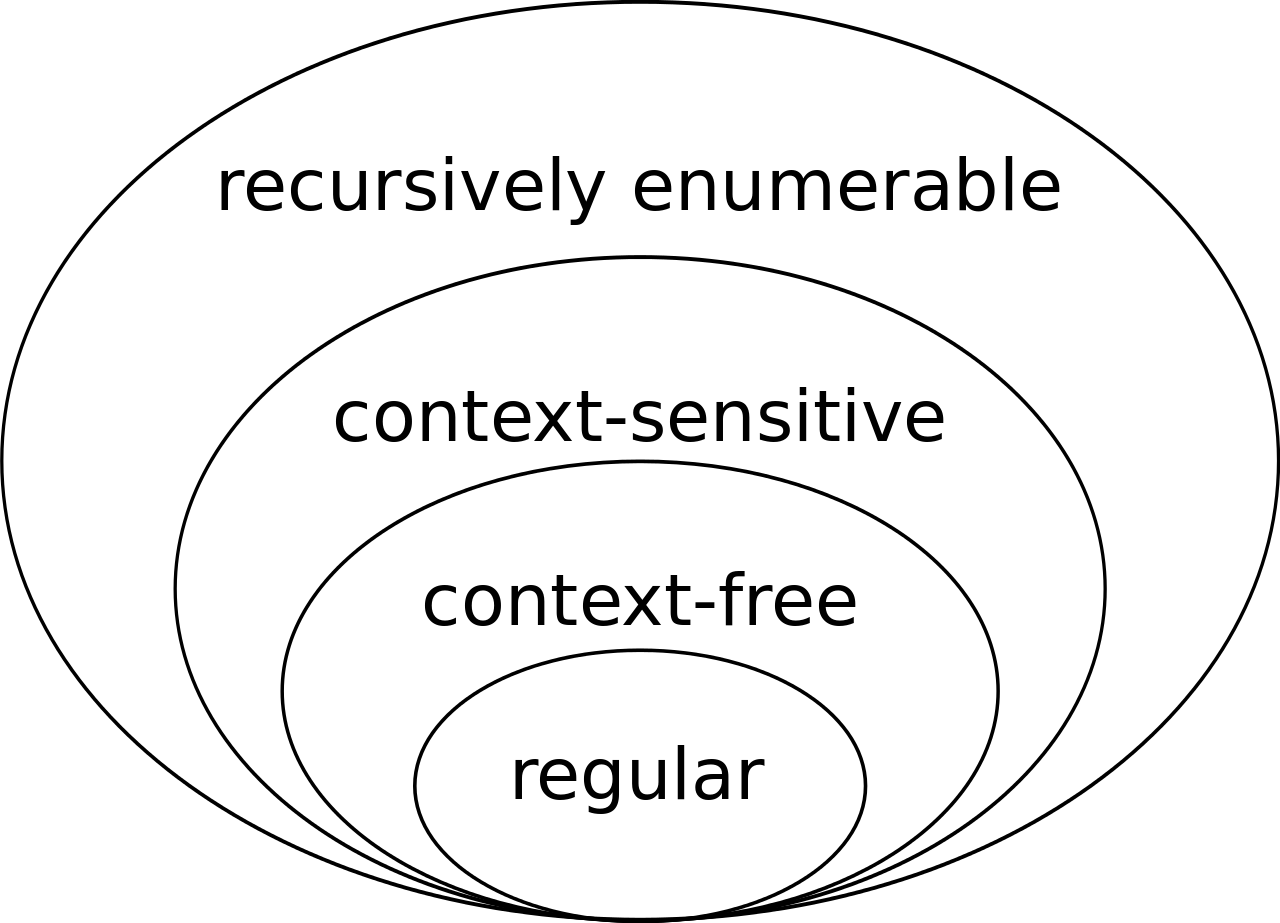
\includegraphics[width=0.5\textwidth]{img/Chomsky.png}}
    \caption{\hierarchy{}, by J. Finkelstein}
    \label{fig:Chomsky}
\end{figure}

\subsection{Using \hierarchy{} \\within a compiler}
When discussing about parsing a programming language, it is important to differentiate between the syntax of the language, and the \textit{semantics} of the language. As confusion between the two can lead an individual to believe a language is one type, when it is actually a subset. Compilers when parsing language have a lexical analyser, which would group characters into much more meaningful sequences known as \textit{lexemes}\cite{DragonBook}. This form of lexical analysis, has become a standard being used by a variety of works\cite{CompilerTutorial}\cite{CompilerBasics}\cite{CompilerConstruction}. Lexemes are then converted into a tokens commonly in the form of a key, value pairing. \\ \centerline{(\textit{token-name}, \textit{attribute-value})}

Raw symbols such as digits, or mathematical symbols(\textit{+,-,/,*}) are mapped into their token-name equivalents. Where as variables, the compiler will map the token-name to a token representing that it is an identifier eg. \textit{id, ident, identifier}. What defines what is a symbol, and what is a identifier is solely up to the \compiler{} writer's decision. The compiler will then assign the attribute-value to number representing it's key in the Symbol-Table. The Symbol-Table is designed to contain much more concrete information about the token, such as it's name, and it's type e.g. \textit{``int, float, double, string''}. The set of tokens is then passed to the syntax analyser.

The syntax analyser will only look at the token-name getting only a vary abstract representation of the code, and can only report syntactical errors such as using wrong keywords, or having incorrect mathematically expressions eg $x = 1 + - + 1$. This is shown clearly in Figure~\ref{fig:invalidC}. Where when run through a C compiler the compiler will print out ``\textit{error: \lq{}x\rq{} undeclared (first use in this function)}''. 
\newpage
This could lead an individual that the syntax of the parser, and thus the language must be context-sensitive, as the compiler knew that ``\textit{x}'' was being used before it existed. The compiler could be using a parsing grammar that is context-free, and the semantic analyser is what determined that the code written was invalid\cite{DragonBook}. As the syntax analyser goes through each token it builds a parse tree, showing the relationship of the tokens as seen in Figure~\ref{fig:AST}. It is solely within the syntax analyser that defines the language type of the programming language.
\begin{figure}[!hbtp]
    \begin{verbatim}
                int main() {
                    x++;
                    int x = 1;
                    return 0;
                }
    \end{verbatim}
    \caption{C code with valid syntax, but invalid semantics.}
    \label{fig:invalidC}
\end{figure}
The semantics of the language are typically defined within a semantics analyser. One common part included within the analyser is \textit{``type checking''}. Where the compiler checks the types on both sides of an operand(\textit{``+,-''}). An common example used is array indexing\cite{DragonBook}. As commonly programming languages require the index number to be an integer eg. array[1], not array[1.5].
\begin{figure}[!hbtp]
    \centering
    \begin{tikzpicture}
        \tikzset{every tree node/.style={align=center,anchor=north}}
        \Tree[.= [.x \textit{id} {} ] 
                 [.+  
                     [.1 ] 
                     [.- {}  
                         [.+ {} 
                             [.1 ] 
                         ] 
                     ]  
                 ] 
             ] 
    \end{tikzpicture}
    \caption{An Abstract Syntax Tree.}
    \label{fig:AST}
\end{figure}
\newpage
Once the syntax of the language is decided the next important step is to determine the parse method. Parsing methods commonly fall into two categories \textit{Top-down}, and \textit{bottom-up}. top-down parsing's popularity is due to the fact that it is easier to write by hand\cite{DragonBook}. Top-down parsing is however typically slower, and requires more memory than bottom-up parsing. However writing a bottom-up parser by hand is so difficult, that most bottom up parsers are generated by parser generator tools.


\textit{Lex} \& \textit{Yacc} are typically recommended for generating code from formal grammars that were discussed earlier\cite{DragonBook}. Both of these tools are available by default in most UNIX based Operation Systems. \textit{``Lex \& Yacc''} argues that creating parsers using the tools will produce much more concise, clear, and bug-free code than writing the parser by hand\cite{LexYacc}. Lex uses regular expressions, and thus can only however generate \textit{regular languages}, which cannot handle nested grammars.

Yacc however uses \textit{grammars} like those shown in \ref{fig:grammar}, and can be used to generate the other types of languages where Lex fails. Both of these tools can only generate C programs. This is a very limiting aspect of both, and could be considered a non starter for building a parser for those who don't wish to use, or do not have experience in developing C programs. There are however plenty of forks(where fork means when a developer takes a copy of the source code, and starts independent development\cite{Fork}) of the tools designed to generate different programming languages' as output.
\newpage
When writing a top-down parser, the most common method is \textit{``recursive descent''}\cite{DragonBook}\cite{ParseTech}. \textit{``Recursive descent parsing''} is the method of defining a set of recursive procedures, where each procedure is associated with each \textit{``nonterminal''} of the grammar. This method however is not foolproof, and can infinitely recurse\cite{DragonBook}. This is shown in Figure \ref{fig:leftR} where the head of the production rule is the same as the nonterminal of the rule, and since in recursive descent the symbol that the parser is currently using is only changed when there is a match, and no matches occur until the recursion ends. The program will loop infinitely.

\begin{figure}[!hbtp]
    \begin{align*}
        expr &\rightarrow\ expr + term
    \end{align*}
    \caption{A example of Left Recursion\cite{DragonBook}}
    \label{fig:leftR}
\end{figure}
\textit{Bottom-up parsing} is the method of instead of beginning at the root, of a parse tree, and working through to the \textit{leaves}(A node within a tree that has no children). Bottom-up parsing instead begins at the leaves, and works up to the root of a tree. The most common method within the Bottom-up approach is \textit{shift-reduce parsing}. This is where the parse has a stack, of all grammar symbols, and an input where the rest of the string that is waiting to be parsed into the stack is held. This method is typically very complicated to write by hand. It is recommended to use an automatic grammar generator instead, such as Lex \& Yacc.


\section{Conclusion}
In conclusion, when building a parser the most important first step, is determining the grammar and syntax of the language. The use of tools like Lex, and Yacc, can help with that initial process. And can help build efficient parsers. However, if the desire is to write a Type 0, or Type 1 language the programmer may be required to write it by hand, which can cause the parse to be slower, and the complexity of type 0, and type 1 hierarchies would discourage most from using them.

